\subsection{Bluez The official Linux Bluetooth stack}
\textbf{BlueZ} is the official Linux Bluetooth protocol stack. It is an Open Source project distributed under the GNU General Public License (GPL). BlueZ kernel is part of the official Linux kernel since version 2.4.6.
\begin{figure}[ht]
	\centering
	
\includegraphics[width=3.5in, height=3in]{images/bluez_intro.png}
	\caption{Bluez the official Bluetooth stack of Linux}
\end{figure}
\subsubsection{History}
The Bluetooth technology was announced in May 1998 with the goal to create an easy usable cable replacement. But Bluetooth has proven to be more than a simple cable replacement technology with an enormous scope of applications and a rich set of standard protocol suite. The first steps into supporting Bluetooth with Linux were done by Axis Communications with their OpenBT Bluetooth Stack in April 1999. Also IBM released its BlueDrekar which was only available as binary modules. The problem of both stacks was that they are character driven, but the Bluetooth technology is for connecting devices. So it is better to integrate it into the Linux network layer and to use the socket interface as primary API.\\
On May 3, 2001, the Bluetooth protocol stack called BlueZ which was written by Qualcomm was released under GPL. The new stack followed the socket based approach. A socket in network programming represents the endpoint of a communication link. The idea is that from a software application's point of view, all data being passed through the link must go into or come out of the socket. Later it was picked up by Linus Torvalds and integrated into the Linux 2.4.6-pre2 kernel. This led to the Open Source community to support BlueZ as official Bluetooth Protocol Stack for Linux.
\subsubsection{The Bluetooth Stack}
The Bluetooth Stack is divided into three components.
\begin{enumerate}
	\item The controller
	\item The Host
	\item The Application
\end{enumerate}
Another important component is the Host Controller Interface.
\begin{figure}[ht]
	\centering
	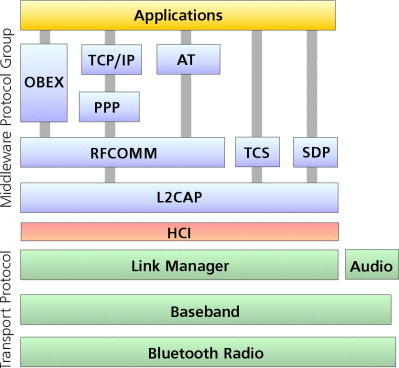
\includegraphics[scale=0.5]{images/bluetooth_stack.png}
	\caption{The Bluez Stack}
\end{figure}
The whole Bluetooth Stack has been divided into two component stacks in Linux. One portion of the stack is made part of the kernel space. The other portion is available as a separate toolkit for the users in the user-space.
\begin{figure}[ht]
	\centering
	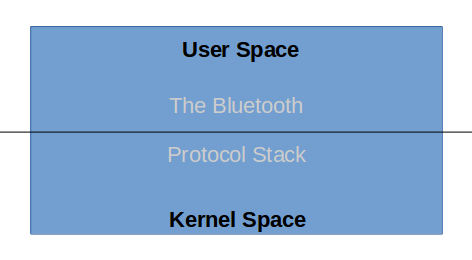
\includegraphics[width=3.5in, height=3in]{images/kernel_userspace.png}
	\caption{Stack division}
\end{figure}
The source for all of the kernel side code can be located in the Linux kernel at: \textbf{/net/Bluetooth}.\\
The Kernel side of the stack contains:
\begin{itemize}
	\item Low level protocols (L2CAP, RFCOMM, BNEP, HIDP, etc)
	\item Security (SSP, SMP)
	\item Hardware drivers
	\item Provides socket based interfaces to user space
	\begin{itemize}
		\item For data (L2CAP, RFCOMM, SCO, HCI)
		\item For control (MGMT, HCI, BNEP, HIDP)
	\end{itemize}
\end{itemize}
The source for the user-space side of Blue can be ne obtained from \textbf{http://www.bluez.org/download/}. It consists of the following things:
\begin{itemize}
	\item Bluetoothd
	\begin{itemize}
		\item Central daemon
		\item D-Bus interfaces for UI and other subsystems
		\item Reduces exposure to low details
		\item Extendible with plugins (eg neard for NFC)
	\end{itemize}
	\item Obexd
	\begin{itemize}
		\item Daemon for OBEX profiles
		\item D-Bus interface for UI
		\item Similar architecture to bluetoothd
	\end{itemize}
	\item Tools
	\begin{itemize}	
		\item Bluetoothctl – command line agent
		\item Btmon -HCI tracer
		\item Set of command line tools useful for testing, development and tracing
	\end{itemize}
\end{itemize}
The whole Bluez architecture is summed up by the following figure:
\begin{figure}[ht]
	\centering
	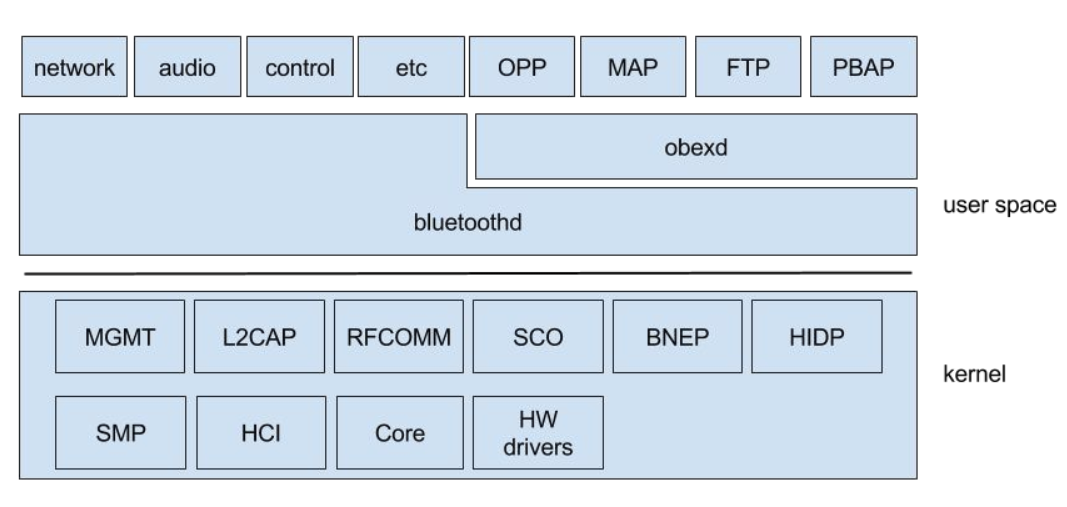
\includegraphics[width=3.5in, height=3in]{images/whole_bluez.png}
	\caption{The whole Bluez Stack}
\end{figure}
